\chapter{Motivação e objetivos}\label{chap:problema}

Este capítulo apresenta a motivação do trabalho, a delimitação do problema de pesquisa, a justificativa e os objetivos que orientam a proposta. A organização segue a recomendação de que a motivação explique o problema real abordado e de que os objetivos sejam verificáveis ao longo da metodologia \citep{WAZLAWICK2020}.

\section{Motivação}

A agricultura tem incorporado tecnologias digitais para lidar com desafios relacionados à produtividade, uso eficiente de recursos, variabilidade climática e acompanhamento de grandes áreas de produção. Em muitas propriedades, o monitoramento da lavoura ainda depende de vistorias presenciais, relatórios manuais ou ferramentas comerciais de custo elevado. Esse cenário pode limitar o acesso de pequenos produtores, estudantes e pesquisadores a informações objetivas sobre a condição da vegetação ao longo do ciclo produtivo.

O sensoriamento remoto oferece uma alternativa relevante para esse problema, pois permite observar a superfície terrestre sem contato físico direto, utilizando sensores embarcados em satélites. Imagens multiespectrais possibilitam a análise de bandas que não são percebidas pelo olho humano, como o infravermelho próximo e o infravermelho de ondas curtas. A partir dessas bandas, é possível calcular índices espectrais que resumem características da vegetação, como vigor, densidade e teor de umidade.

\begin{figure}[htb!]
    \centering
    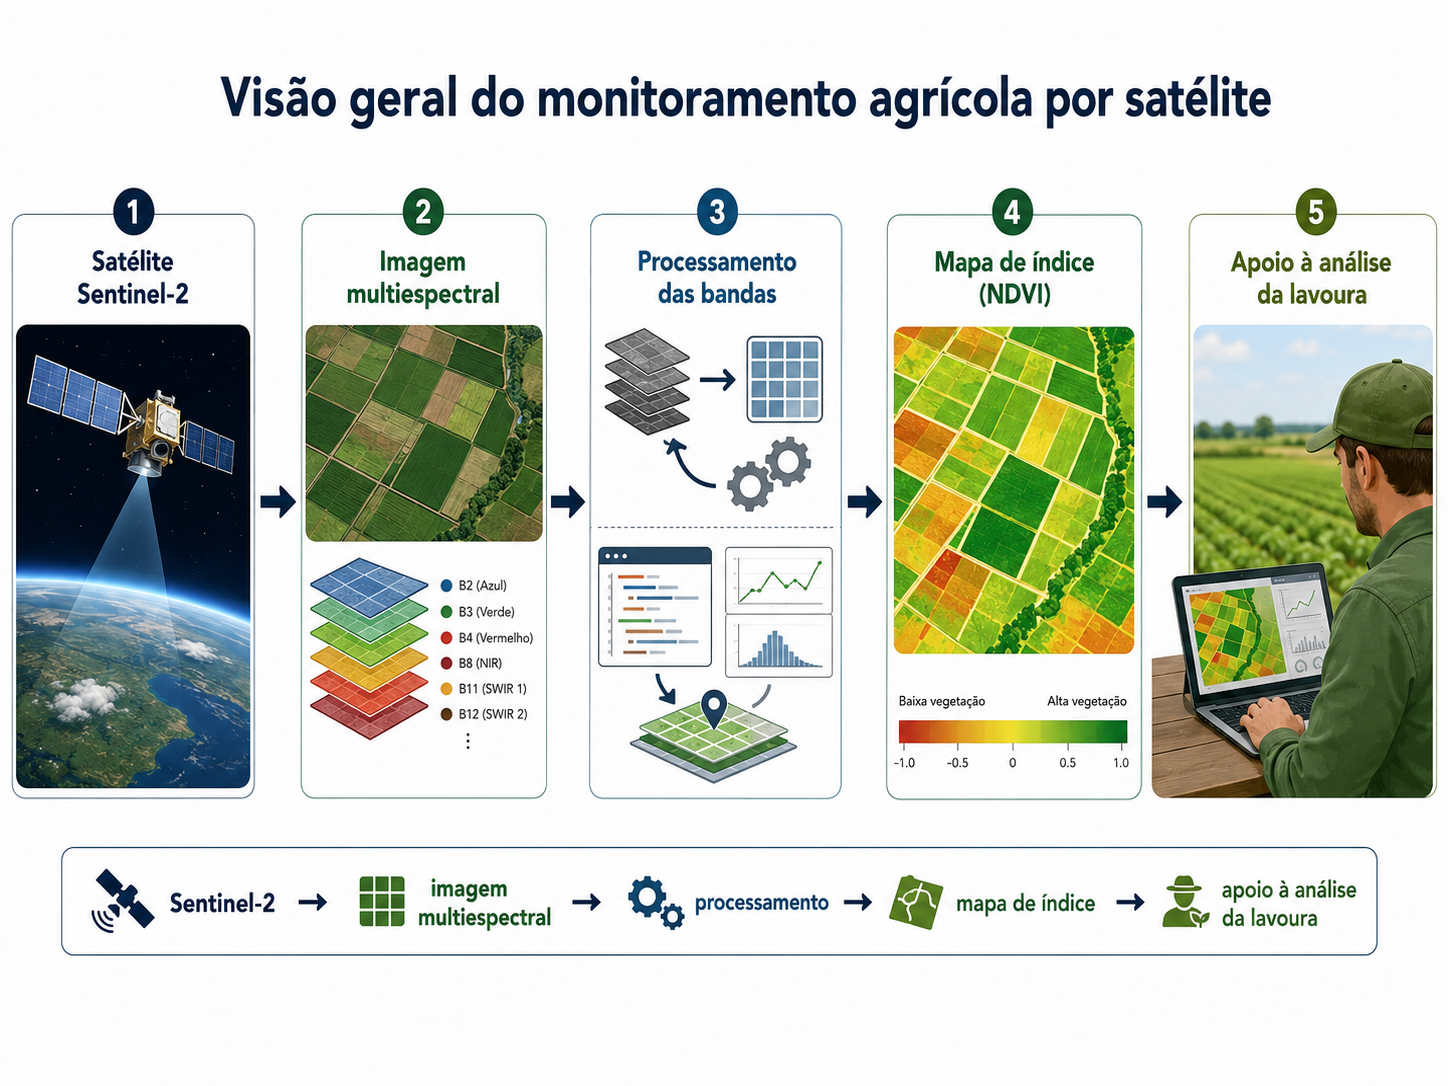
\includegraphics[width=0.92\textwidth]{fig/figura1.png}
    \caption{Visão geral do uso de imagens de satélite no monitoramento agrícola.}
    \label{fig:visao-geral-monitoramento}
    \vspace{0.2cm}
    \small Fonte: Elaborado pelo autor (2026).
\end{figure}

Entre os índices mais utilizados está o \textit{Normalized Difference Vegetation Index}, conhecido como NDVI, que relaciona a reflectância no vermelho e no infravermelho próximo para estimar o vigor da vegetação \citep{ROUSE1973}. Para complementar essa análise, o \textit{Normalized Difference Water Index}, conhecido como NDWI na formulação voltada ao teor de água da vegetação, utiliza bandas no infravermelho próximo e no infravermelho de ondas curtas \citep{GAO1996}. A combinação desses índices permite observar tanto a condição geral da vegetação quanto possíveis sinais de estresse hídrico.

A disponibilidade de imagens Sentinel-2 e o acesso a plataformas como Google Earth Engine tornam possível processar grandes volumes de dados geoespaciais sem exigir armazenamento local de imagens \citep{GOOGLE_S2_SR}. Além disso, a função de diferença normalizada do Earth Engine apoia a implementação direta dos índices espectrais previstos \citep{GOOGLE_EE_ND}. Bases climáticas como NASA POWER podem ser utilizadas para relacionar alterações nos índices espectrais com precipitação, temperatura e radiação solar \citep{NASA_POWER_DAILY}. Dessa forma, há uma oportunidade de desenvolver um sistema acadêmico simples, de baixo custo e reproduzível, capaz de demonstrar a aplicação prática de sensoriamento remoto no monitoramento agrícola.

A motivação deste trabalho está na necessidade de aproximar técnicas de sensoriamento remoto e ciência de dados de um protótipo acessível, voltado à visualização de mapas, séries temporais e alertas preliminares. O sistema proposto não pretende substituir a inspeção em campo nem fornecer diagnóstico agronômico definitivo. Seu propósito é apoiar a análise inicial da lavoura, indicar regiões ou períodos que merecem atenção e demonstrar a viabilidade do uso de dados gratuitos no contexto do agronegócio.

\section{Problema de pesquisa}

O problema abordado por este trabalho pode ser formulado da seguinte maneira: como desenvolver um sistema de baixo custo, baseado em imagens de satélite e dados climáticos gratuitos, capaz de auxiliar no monitoramento da condição da vegetação em áreas agrícolas por meio de índices espectrais e séries temporais?

Esse problema envolve aspectos computacionais e metodológicos. Do ponto de vista computacional, é necessário integrar interface, processamento geoespacial, APIs externas, cálculo de índices, geração de mapas e visualização temporal. Do ponto de vista metodológico, é preciso definir quais dados serão utilizados, como os índices serão calculados, quais critérios serão adotados para detectar anomalias e como os resultados serão validados.

\section{Justificativa}

A justificativa técnica do trabalho está na possibilidade de integrar tecnologias consolidadas, como Python, Streamlit, Google Earth Engine, Sentinel-2 e NASA POWER, em um fluxo único de análise. Essa integração permite construir um protótipo que processa dados reais e apresenta resultados compreensíveis ao usuário, sem exigir infraestrutura complexa.

A justificativa acadêmica está na aplicação de conceitos de Ciência da Computação a um problema interdisciplinar, envolvendo desenvolvimento de software, processamento de dados, visualização, geoprocessamento e validação experimental. O trabalho também contribui para demonstrar como um sistema computacional pode organizar dados de sensoriamento remoto e clima em uma ferramenta de apoio à análise agrícola.

A justificativa social e prática está relacionada à democratização do acesso a informações sobre lavouras. Embora existam soluções comerciais avançadas, nem sempre elas são acessíveis para pequenos produtores ou ambientes educacionais. Um protótipo baseado em ferramentas gratuitas pode servir como base para estudos, treinamentos, pesquisas futuras e evolução para aplicações mais robustas.

\section{Objetivo geral}\label{sec:obj_geral}

Desenvolver um sistema de monitoramento agrícola baseado em imagens de satélite, capaz de calcular índices espectrais, gerar mapas e séries temporais e indicar possíveis anomalias na vegetação, demonstrando a viabilidade do uso de sensoriamento remoto e ferramentas gratuitas como apoio à análise de áreas cultivadas.

\section{Objetivos específicos}\label{sec:obj_espec}

Para alcançar o objetivo geral, foram definidos os seguintes objetivos específicos:

\begin{itemize}[leftmargin=3em]
    \item estudar conceitos de sensoriamento remoto aplicados ao monitoramento agrícola;
    \item investigar o uso de imagens Sentinel-2 para análise de vegetação em áreas cultivadas;
    \item definir a arquitetura do sistema, integrando interface, processamento e fontes externas de dados;
    \item implementar rotinas em Python para consulta de imagens no Google Earth Engine;
    \item calcular índices espectrais, com foco em NDVI e NDWI, a partir das bandas do Sentinel-2;
    \item gerar mapas temáticos e séries temporais dos índices calculados;
    \item integrar dados climáticos da NASA POWER para análise complementar;
    \item implementar mecanismo simples de detecção de anomalias com base em desvio estatístico;
    \item desenvolver interface web em Streamlit para entrada de parâmetros e visualização dos resultados;
    \item validar o protótipo com áreas agrícolas representativas, como soja, milho e pastagem;
    \item documentar limitações, resultados esperados e possibilidades de evolução do sistema.
\end{itemize}

\section{Hipóteses e pressupostos de validação}\label{sec:hipoteses}

Como se trata de uma proposta de desenvolvimento de protótipo, a validação será orientada principalmente pelo atendimento aos objetivos e pelo comportamento esperado do sistema. Ainda assim, serão considerados os seguintes pressupostos:

\begin{itemize}[leftmargin=3em]
    \item o uso de imagens Sentinel-2 permite obter séries temporais úteis para observar variações de vegetação em áreas agrícolas;
    \item a combinação entre NDVI e NDWI oferece uma visão mais completa do estado da lavoura do que o uso isolado de apenas um índice;
    \item a integração com dados climáticos auxilia na interpretação de quedas ou oscilações dos índices espectrais;
    \item um protótipo baseado em ferramentas gratuitas é suficiente para demonstrar a viabilidade técnica da abordagem em contexto acadêmico.
\end{itemize}
